\documentclass[uplatex,10pt,a4paper,twocolumn]{jsarticle}
%
\usepackage{amsmath}
\usepackage{bm}
%
\def\diff{\mathrm d}
\def\dd#1#2{\dfrac{\diff #1}{\diff #2}}
\def\pp#1#2{\dfrac{\partial #1}{\partial #2}}
\def\dd2#1#2{\dfrac{\diff^2 #1}{\diff #2^2}}
\def\pp2#1#2{\dfrac{\partial^2 #1}{\partial #2^2}}
%
\usepackage[dvipdfmx]{graphicx, color}
%
\pagestyle{empty}
\usepackage[truedimen,margin=25truemm]{geometry}

\renewcommand{\baselinestretch}{0.87} % 全体の行間調整
\renewcommand{\figurename}{Fig.}
\renewcommand{\tablename}{Tab.}
\usepackage{setspace}

\graphicspath{{../../figures/}}

\begin{document}
\twocolumn[

\begin{center}
{\Large MD シミュレーションによるネットワークポリマーの緩和挙動}
\end{center}
\begin{flushright}
{\large 東亞合成  $\bigcirc$佐々木裕}
\end{flushright}

%\vspace{1mm}

\begin{center}
{\large Relaxation Characteristics of Network Polymers with random connectivity \\using Molecular Dynamics Simulations}

$\bigcirc$H. Sasaki\\
Toagosei Co., Ltd
\end{center}
\vspace{2mm}

]


\begin{spacing}{0.9}
ABSTRACT: 
Existence of mechanical hysteresis is believed to be one of a key to achieve high durability for rubber materials.
``Phantom Network Model'', in which fluctuation of junction point is rather high, seems to be a good candidate for micro-scale energy dissipation.

Employing molecular dynamics simulation method, relaxation characteristics of ``Phantom Network Model'' was investigated.
\end{spacing}

\section{はじめに}
% \subsection{しなやかなネットワークポリマー}

% 省エネルギーの観点から自動車を中心とした輸送機器の大幅な軽量化の検討が進められており、その中でCFR(T)Pをはじめとする多様な新素材を用いたマルチマテリアル化の鍵の一つとして接着接合技術が注目されている。
% % 接着剤の主成分には、1分子中に複数の反応性官能基を有する反応性オリゴマーが用いられており、光や熱などの外部刺激により速やかにネットワーク構造を形成し、優れた機械的特性を示す。
% この場合、接着剤として使用されるネットワークポリマーに要求される特性は、一次的な機械的物性が高いだけでなく、長期間の使用における耐久性を確保するために、さまざまな変形速度で繰り返し変形させる疲労試験に耐えることが要求される。このような考え方から、脆性破壊を起こしやすい硬い機械物性ではなく、しなやかな強度と延性を兼ね備えたネットワークポリマーが注目されている。

% \subsection{力学的ヒステリシスの重要性}

% 材料の耐久性を確保するためには機械的性質の発現機構とその劣化メカニズムを解明する必要があり、金属などのハードな材料では破壊工学として体系化されている。
% 破壊工学の概念を端的に表現すると、「系内に欠陥が存在することを前提とした耐久性の評価」である。破壊挙動は、材料の脆性破壊を仮定した「グリフィス理論」における亀裂進展に伴うエネルギー放出速度である$G_c$と、$J$積分により非線形領域に拡張された$J_c$で議論され、これらの値が靭性の指標とされている。
% しかし、破壊時の変形が極めて大きいソフトマター材料への適用には注意が必要である。

旧知のソフトな材料であるゴムの破壊靭性が大きい原因として、その破壊エネルギーが応力-ひずみ関係における機械的ヒステリシスロスと良い相関を示すことが報告されている~\cite{payne1}。
Andrewsは、応力-ひずみ関係における機械的ヒステリシスに着目し、ヒステリシス損失によりき裂進展に伴うエネルギー放出が減少し、結果としてき裂進展が抑制されるというモデルを提案した~\cite{andrews}。
Payneは、ヒステリシスロスの発現機構を、1) 粘弾性に基づくもの、2) 結晶化に基づくもの、3) フィラー添加によるもの、の3つの主要なメカニズムに分類した~\cite{payne2}。
ヒステリシスの原因として、フィラー由来、あるいは、伸張結晶化のようなメゾスケール領域の挙動に注目する場合が多く見受けられる~\cite{zhang}。
また、超高強度ゲルとして知られているダブルネットワークゲル中の犠牲結合においても、大きなヒステリシスが見られる~\cite{gong}。
このような検討は分子鎖の描写よりもわずかに大きいメソスケール領域に注目しており、この比較的大きなスケールでの挙動は、一般に遅い緩和時間をもたらす。
% ヒステリシス挙動はこのスケールでのみ起こるのだろうか?
また、破壊試験による材料の強度評価は任意の変形速度での一回の変形挙動で評価されるため、ヒステリシスの回復挙動の遅速はあまり問題にならない。
しかしながら、材料としての耐久性を保証するためには、多様な変形速度での繰り返し変形を行う疲労試験に対する耐久性も重要である。
この場合、適正な緩和時間で回復する可逆的なメカニズムに基づく強靭化機構が必要となり、それに対応しうる機械的ヒステリシスの設計が望まれることとなる。

このような観点から、エントロピー弾性であるゴム弾性のモデルについて考えてみよう。
ゴム弾性の古典的なモデルである ``Affine Network Model'' からの発展形として、結節点の揺らぎに注目した``Phantom Network Model: PNM''が提案され、Flory によればメルト状態と同一なストランドのゆらぎを有するランダムネットワークにおいて PNM のふるまいを示すとされている~\cite{flory}。
また、ゴム系材料の破壊において時間温度換算則が大変形を伴う破壊挙動にも成立し、室温では容易に破断する SBR がガラス転移温度に近い低温での伸長では高い伸びと強度を示すことも報告されている~\cite{smith}。
我々は、この結節点のゆらぎ由来の散逸が、分子鎖描像のようなミクロなスケールでの粘弾性的なエネルギー散逸モデルとなりうるのではないかと考え、これまで検討を進めている~\cite{sasaki}。




% \subsection{目指すもの}




% \subsection{本検討内容}
% (本検討内容)
ソフトマターの構造材料への展開を標語的に言えば、「脆性破壊を伴いがちな剛直性から、設計された延性に基づく高耐久性を示す『しなやかな強さ』へのパラダイムシフト」となるであろう。
この設計された延性に必要な要件を明確にすることが本研究の目的である。
本報告では、ランダムな接続性を有するネットワークポリマーを用いて、その力学特性と緩和挙動との関係について、MD シミュレーションにより検討した結果について報告する。




\section{シミュレーション}
既報~\cite{sasaki}に従い、任意の分岐数$f$($f=3\sim6$)の結節点からなるランダムな接続性を有するネットワークを作成し、その平衡状態および変形(一軸伸張およびずりせん断)時の振る舞いについて、OCTA 上の COGNAC シミュレーターを用いた分子動力学シミュレーションにより評価した。

\subsection{ネットワークモデルの作成}
トポロジーモデルの「代数的連結性」を指標として以下のアルゴリズムでランダムな結合性を導入した。
% \vspace{-2mm}
\begin{enumerate}
\item
実空間での初期構造を体心立方構造の各格子点をストランドでつないだ「八本鎖モデル」として、それに対応するように任意の分岐数のトポロジーモデルを作成。
% (Fig. \ref{fig:topo})。
\item
代数的連結性を指標としてストランド交換し、結節点の結合性にランダム性を導入。
% (Fig. \ref{fig:exc})。
\item
そのトポロジーモデルに対応するように、実空間の初期構造からストランドを除去。
\end{enumerate}

% \subsection{初期構造の作成}
% 任意のセグメント数のストランドを用いてストランドの末端間距離がホモポリマーメルトと同等になるようにユニットセル長と多重度を調整し、KG 鎖の一般的な密度 ($\rho$=0.85) となるモデルを作成した。

\subsection{MD シミュレーション}
排除体積効果を無視してす抜けとした Phantom 鎖、および、セグメント間の非結合ポテンシャルに斥力($r_c = 2^{1/6}\sigma$)である LJ ポテンシャル $U_{LJ}(r_{ij})$、ボンドポテンシャルには FENE-LJ ポテンシャルを用いることで絡み合いを再現した KG 鎖をストランドとしてそれぞれ検討した。
なお、初期構造の緩和は Auhl 等の方法~\cite{Auhl} に従い force-capped-LJ ポテンシャルを用いて、段階的にす抜け鎖から絡み合い鎖へと遷移させた。
% 初期緩和終了後に、Kr\"{o}ger らの方法~\cite{Kroger} によりストランド同士の絡み合いを評価して、対応するホモポリマーメルトと同程度であることを確認した。
% また、密度の低い初期状態から NPT 計算により圧縮することで、絡み合いを極力排除した比較計算も実施した。

\section{結果と考察}

\subsection{PNMの確認}
同一のストランド長(セグメント数: 50)を有する 3, 4, 6 分岐のネットワークポリマーにおける変形速度依存性が消失するせん断変形($\dot{\gamma} \simeq 5e^{-6}$)での SS カーブ(Fig. \ref{fig:shear})はほぼ線形応答となった。
PNM から予想される値よりも高い弾性率は Trapped Entanglement を考慮したモデルで説明できた~\cite{rubinstein}。
\vspace{-3mm}
\begin{figure}[htb]
\centering
	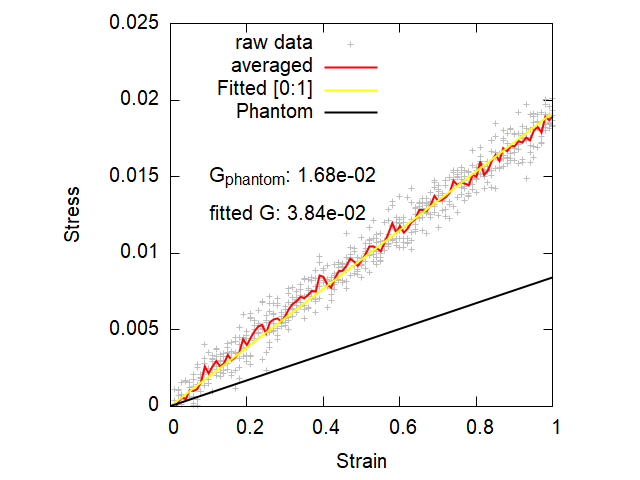
\includegraphics[width=.47\textwidth]{4chain_N50_shear.png}
	\caption{Stress-Strain Curves for 4-chain NW at shear rate: $\dot{\gamma} = 5e^{-6}$}
	\label{fig:shear}
\end{figure}
\vspace{-5mm}

\subsection{粘弾性スペクトル}
ステップ変形による応力緩和関数 $G(t)$ より導出した動的粘弾性スペクトルを Fig. \ref{fig:spectrum} に示した。
$\tan \delta$ は上述の変形速度依存性が消失する程度の時間スケールで減衰したが、同等な長さのホモポリマーの最長緩和時間よりは長時間化していた。

この緩和時間の長時間化はネットワーク構造に起因した架橋点の運動性の低下によるものと想定でき、長鎖のホモポリマーメルトでの絡み合いに起因したラウスモードのふるまい~\cite{kalathi} と合致していた。


\subsection{ヒステリシスロスの速度依存性}

4分岐のネットワークに周期的なせん断変形 ($\gamma = 1$, $\dot{\gamma} = 5e^{-5}$) を付与した結果を Fig. \ref{fig:hystloss} に示した。
複数回の変形に対しても迅速な回復を伴った力学的ヒステリシス (Hysteresis loss $\simeq$ 0.36) を示すことが確認できた。

\vspace{-3mm}
\begin{figure}[htb]
\centering
	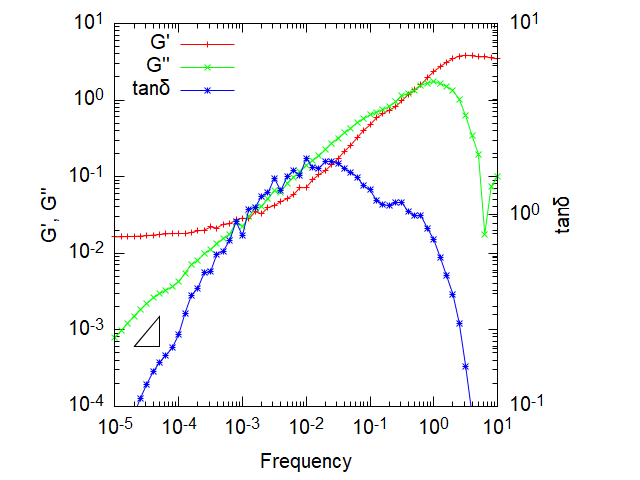
\includegraphics[width=.47\textwidth]{gw_4chain_N50_stepstretch.png}
	\caption{Linear dynamic visco-elastic spectrum for 4-chain NW(N=50)}
	\label{fig:spectrum}
\end{figure}
\vspace{-5mm}

\vspace{-3mm}
\begin{figure}[htb]
\centering
	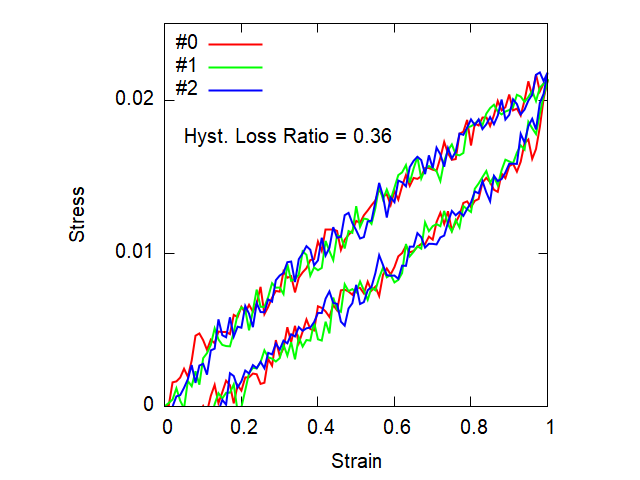
\includegraphics[width=.47\textwidth]{CyclicDeform_4chain_N50_rate5e-5.png}
	\caption{Hysteresis Curves for 4-chain NW(N=50) by Cyclic Shear($\gamma = 1$, $\dot{\gamma} = 5e^{-5}$)}
	\label{fig:hystloss}
\end{figure}
\vspace{-5mm}

\begin{thebibliography}{99}
    \bibitem{payne1} K. Grosch, J.A.C. Harwood \& A.R. Payne, Nature, 212 5061 497 (1966)
    \bibitem{andrews} E. H. Andrews, Y. Fukahori, J. of Mat. Sci., 12, 1307 (1977)
    \bibitem{payne2} A. R.Payne, J. Polym. Sci. Part C, Polym. Symp., 48(48), 169 (1974)
    \bibitem{zhang} H. Zhang et al. Macromolecules 46, 900 (2013)
    \bibitem{gong} J.P. Gong, Soft Matter, 6, 12, 2583 (2010)
    \bibitem{flory} P. J. Flory, Proc. R. Soc. London. Series A, 351, 351 (1976)
    \bibitem{smith} T. L. Smith, R. A. Dickie, J. of Polym. Sci. A-2: Polym. Phys., 7, 635 (1969)
    \bibitem{sasaki} 佐々木裕, 第69回レオロジー討論会 (2021)
    \bibitem{Auhl} R. Auhl et al., J. of Chem. Phys., 119, 12718 (2003)
    % \bibitem{Kroger} S. Shanbhag, M. Kr\"{o}ger, Macromol. 40 2897 (2007)
    \bibitem{rubinstein} M. Rubinstein, S. Panyukov, Macromolecules, 35, 17, 6670 (2002)
    \bibitem{kalathi} J. T. Kalathi et al., Macromol. 47 6925 (2014)
\end{thebibliography}

\end{document}